\documentclass[brazil]{beamer}
% \usepackage{animate}
\usepackage{graphics} 
\usepackage{subfig}
\usepackage{movie15}
\usepackage[utf8]{inputenc}
\usepackage{enumerate}
\usepackage{default}
\usepackage{graphicx,hyperref,url}


% renomear as palavras de LaTeX com nomes fixos
\renewcommand{\figurename}{\tiny{Figura}} 
\renewcommand{\tablename}{\tiny{Tabela} }

\setbeamertemplate{footline}[frame number]
\usetheme{Berkeley}

\title[Diferenciação Celular]{Diferenciação Celular}

%\subtitle{UFRN}
\institute[UFRN]{\inst{a} Universidade Federal do Rio Grande do Norte - UFRN
\and \inst{b} Disciplina: Bilologia Celular}

%\author[Rennan G.]{Rennan G.; \\\medskip}
\date{31 de Maio de 2016}

\logo{
\includegraphics[scale=0.3]{ufrn.png}}

\setlength{\parindent}{0pt}

\begin{document}

\begin{frame}
   \titlepage 
 \end{frame}

\begin{frame}
  \frametitle{Sumário}

  \tableofcontents
\end{frame}

%%%%%%%%%%%%%%%%%%%%%%%%%%%%%%%%%%%%%%%%%%%%%%%%%%%%%%%%%%%%%%%%%%%%%%%%%%%%%%%%%%%%%%%%%%%%%%%%%%%%%%%%%%%%%%%%%%%%%%%%%%%%%%%%%%%%%%%%%%%%%%%%%%%%%%%%%%%%%%%%%%%%%%%%%%%%%%%%
%%%%%%%%%%%%%%%%%%%%%%%%%%%%%%%%%%%%%%%%%%%%%%%%%%%%%%%%%%%%%%%%%%%%%%%%%%%%%%%%%%%%%%%%%%%%%%%%%%%%%%%%%%%%%%%%%%%%%%%%%%%%%%%%%%%%%%%%%%%%%%%%%%%%%%%%%%%%%%%%%%%%%%%%%%%%%%%%
\section{Introdução}

  \begin{frame}
    \frametitle{Introdução}
    \raggedright  
     Definições:
    \scriptsize
    \begin{itemize}
    \item \scriptsize Durante a evolução dos organismos multicelulares novos mecanismos surgiram para diversificar os tipos celulares coordenar sua produção, além de regular seu 
    tamanho e número, organizá-los em \textcolor{red}{\textit{tecidos funcionais}} e eliminar células estranhas ou envelhecidas 
    \end{itemize}   
  \end{frame}
  
  \begin{frame}
  \frametitle{Introdução}
    \raggedright  
    \begin{itemize}
     \item Diferenciação: capacidade de uma célula se \textcolor{red}{especialiar} em funções especificas.
     \item Potencialidade: capacidade de uma célula de \textcolor{red}{originar outros tipos celulares}.
    \end{itemize}
    \begin{figure}
     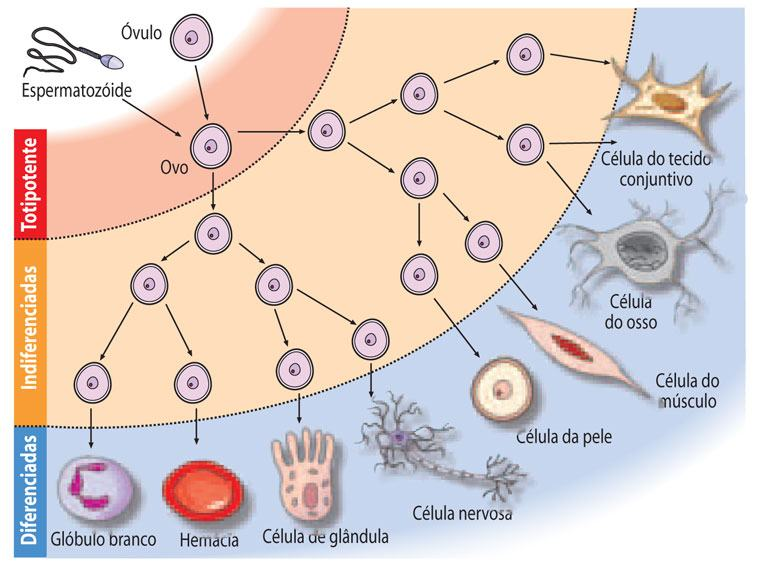
\includegraphics[scale=0.2]{diferenciacao_potencialidade.jpg}
	  \caption{\tiny Inlustração da especialização celular.}
    \end{figure} 
  \end{frame}

  \begin{frame}
  \frametitle{Introdução}
    \raggedright  
    \begin{itemize}
     \item Diferenciação: capacidade de uma célula se \textcolor{red}{especialiar} em funções especificas.
     \item Potencialidade: capacidade de uma célula de \textcolor{red}{originar outros tipos celulares}.
    \end{itemize}
    \begin{columns}[T]
      \begin{column}{0.3\textwidth}
	\begin{itemize}
	  \item Totipotência
	  \item Pluripotência 
	  \item Multipotência
	  \item Unipotência
	\end{itemize}
      \end{column}
      \hfill%
      \begin{column}{0.6\textwidth}
	\begin{figure}
	%\transboxin
	  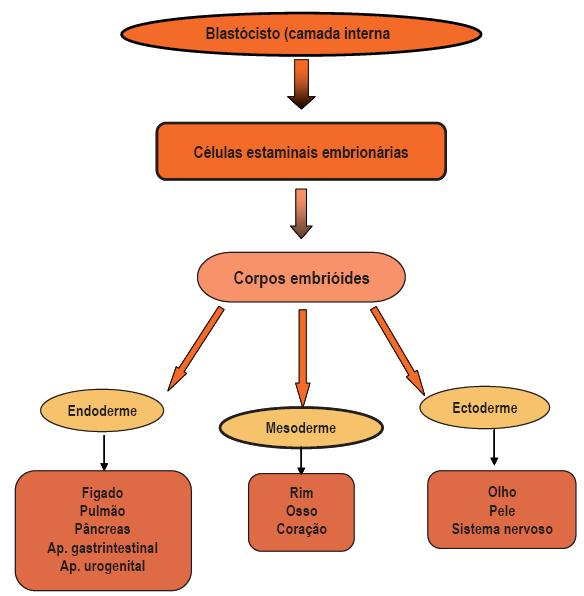
\includegraphics[scale=0.28]{folhetos_embrionarios_2.jpg}
	  \caption{\tiny Vias de diferenciação celular.}
	\end{figure}  
      \end{column}%
    \end{columns}
  
 \end{frame}
  
  \begin{frame}
    \frametitle{Introdução}
    \begin{minipage}{1\textwidth}
	\begin{figure}
	    \centering
	    \subfloat[\label{fig:a}]{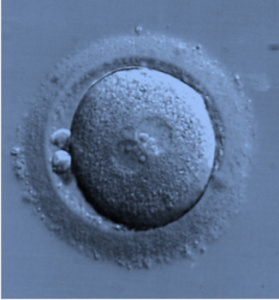
\includegraphics[scale=0.3]{zigoto.jpg}}	  
	    \subfloat[\label{fig:b}]{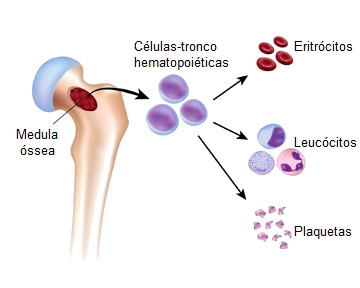
\includegraphics[scale=0.4]{celula_hematopoietica.jpg}}	  
	  \caption{\tiny Potencialidade: \subref{fig:a} Zigoto, Totipotente; \subref{fig:b} Célula Hematopoiética Multipotente;}
	  \label{fig:1}
	\end{figure}
    \end{minipage}
  \end{frame}

  \begin{frame}
    \frametitle{Introdução}
    \raggedright  
    \begin{block}{Modelos Experimentais para estudo:}
     Transplante entre embriões da mesma espécie, em que podemos verificar os efeitos que o microambiente tem sobre a diferenciação
    \end{block}

      \begin{figure}
	  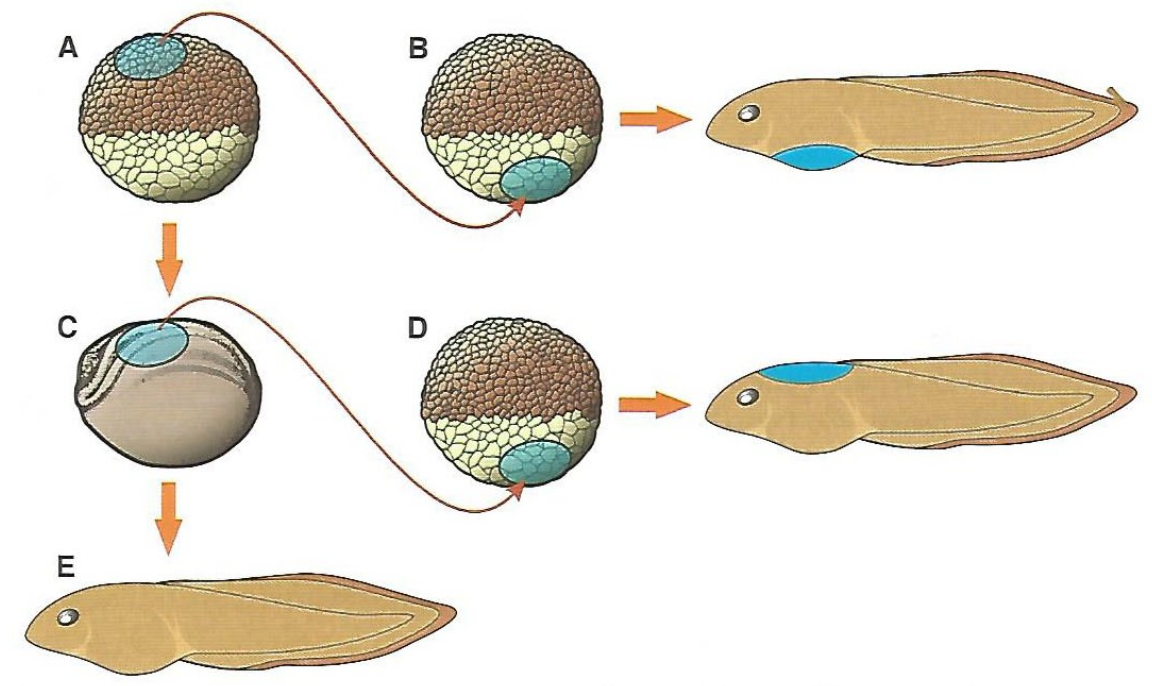
\includegraphics[scale=0.15]{diferenciacao_embrionaria.png}
	  \caption{\tiny Diferenciação Embrionaria, podemos assim verificar uma restrição da plasticidade ou potencialidade celular. Logo, as células mais jovens são mais suscetíveis a sinais extracelulares.}
      \end{figure}
  \end{frame}
  
  \begin{frame}
    \frametitle{Introdução}
    \raggedright  
    \begin{block}{Modelos Experimentais para estudo:}
     As células geralmente selecionam os genes que serão expressados sem alterar a sequência de nucleotídeos do próprio DNA. Por exemplo, células individuais removidas de uma cenoura
    podem regenerar uma planta adulta.
    \end{block}
     
      \begin{figure}
	  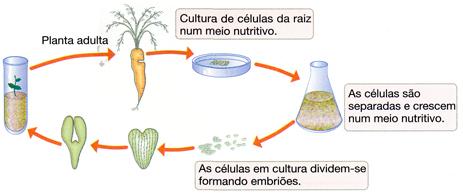
\includegraphics[scale=0.5]{diferenciacao_vegetal.png}
	  \caption{\tiny diferenciação vegetal.}
      \end{figure}
  \end{frame}


%%%%%%%%%%%%%%%%%%%%%%%%%%%%%%%%%%%%%%%%%%%%%%%%%%%%%%%%%%%%%%%%%%%%%%%%%%%%%%%%%%%%%%%%%%%%%%%%%%%%%%%%%%%%%%%%%%%%%%%%%%%%%%%%%%%%%%%%%%%%%%%%%%%%%%%%%%%%%%%%%%%%%%%%%%%%%%%%
%%%%%%%%%%%%%%%%%%%%%%%%%%%%%%%%%%%%%%%%%%%%%%%%%%%%%%%%%%%%%%%%%%%%%%%%%%%%%%%%%%%%%%%%%%%%%%%%%%%%%%%%%%%%%%%%%%%%%%%%%%%%%%%%%%%%%%%%%%%%%%%%%%%%%%%%%%%%%%%%%%%%%%%%%%%%%%%%
\section{Diferenciação}

  \begin{frame}
    \frametitle{Diferenciação}
    \raggedright  
      \begin{itemize}
      \item Clivagem: divisões mitóticas sucessivas. 
      \item Gastrulação: definição dos Folhetos Embrionários
      \end{itemize}
      \begin{figure}
	  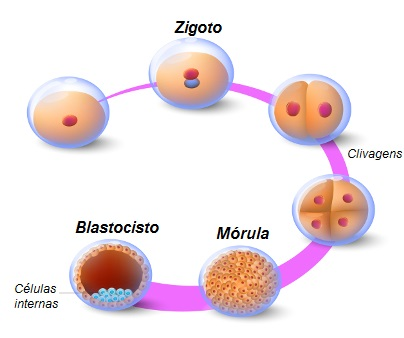
\includegraphics[scale=0.4]{clivagem_zigoto.jpg}
	  \caption{\tiny clivagem zigoto.}
      \end{figure}
  
  \end{frame}

  \begin{frame}  
  \frametitle{Diferenciação}
    \raggedright 
    
    \begin{figure}
      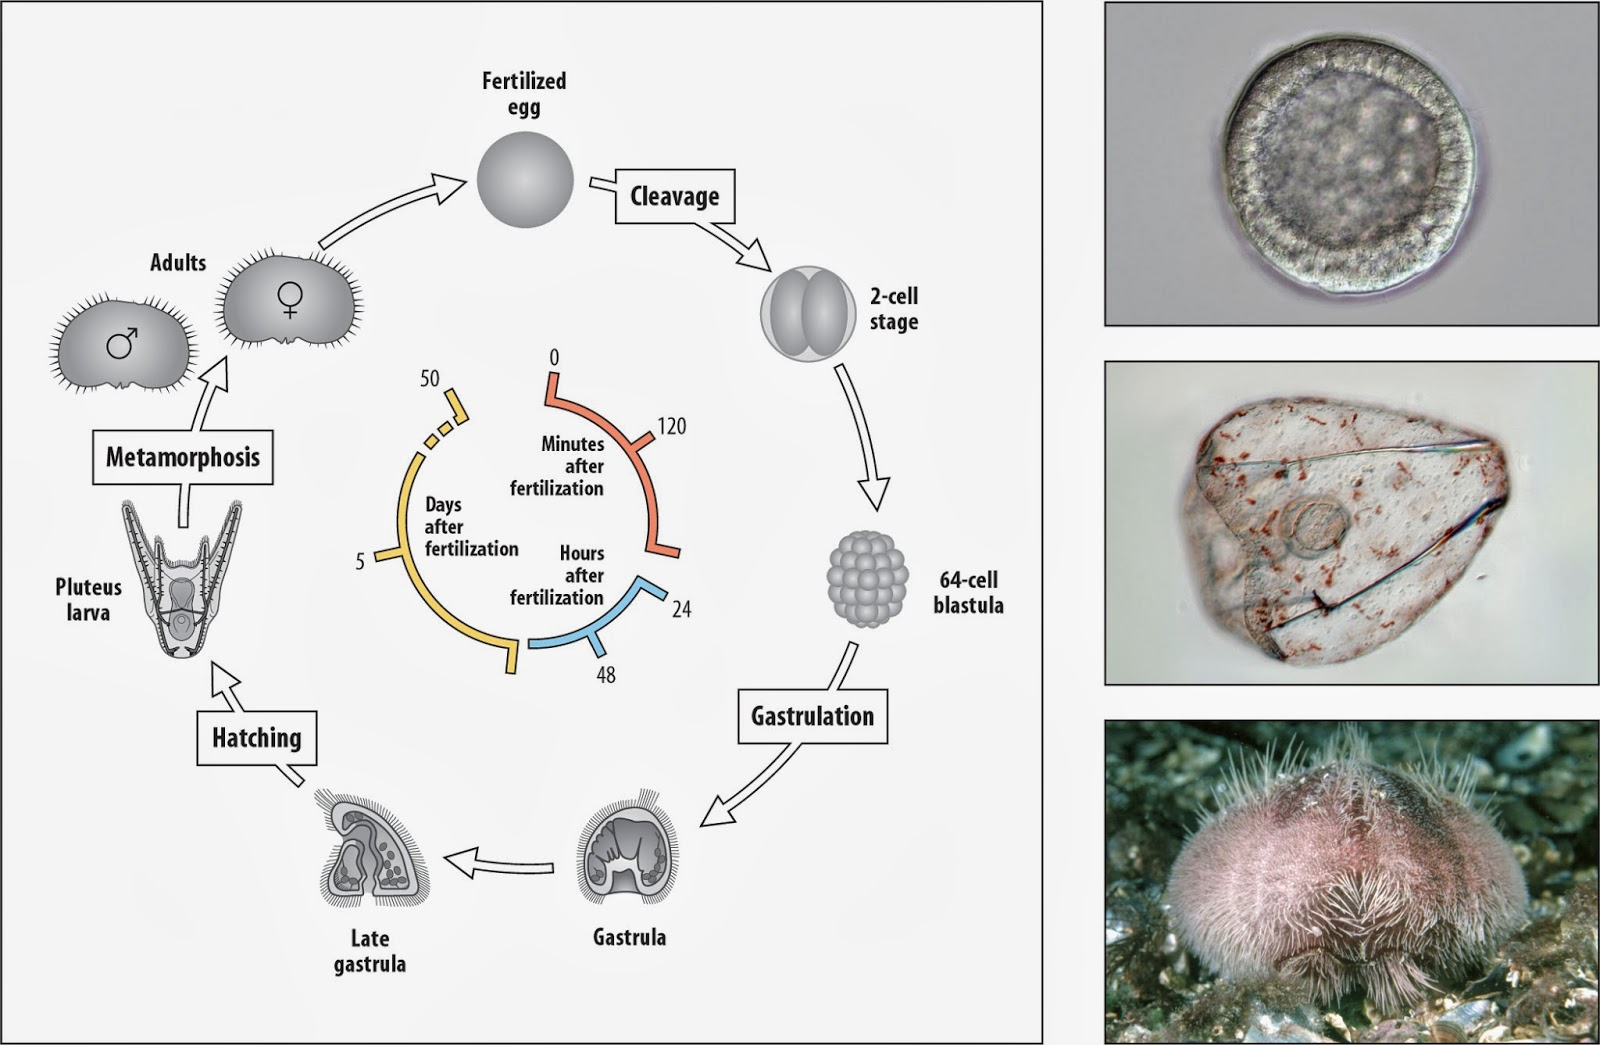
\includegraphics[scale=0.15]{clivagem_ourico_do_mar.jpg}
      \caption{\tiny clivagem ouriço do mar.}
     \end{figure}
  \end{frame}

%%%%%%%%%%%%%%%%%%%%%%%%%%%%%%%%%%%%%%%%%%%%%%%%%%%%%%%%%%%%%%%%%%%%%%%%%%%%%%%%%%%%%%%%%%%%%%%%%%%%%%%%%%%%%%%%%%%%%%%%%%%%%%%%%%%%%%%%%%%%%%%%%%%%%%%%%%%%%%%%%%%%%%%%%%%%%%%%
%%%%%%%%%%%%%%%%%%%%%%%%%%%%%%%%%%%%%%%%%%%%%%%%%%%%%%%%%%%%%%%%%%%%%%%%%%%%%%%%%%%%%%%%%%%%%%%%%%%%%%%%%%%%%%%%%%%%%%%%%%%%%%%%%%%%%%%%%%%%%%%%%%%%%%%%%%%%%%%%%%%%%%%%%%%%%%%%
\section{Controles e Fatores que Atuam na Diferenciação}

\begin{frame}
  \frametitle{Controles e Fatores que Atuam na Diferenciação}
  \raggedright  
  \begin{block}{Expressões Genética:}
    \footnotesize 
      \begin{itemize}
     \item Ação dos Genes: As modificações celulares, que tem lugar na diferenciação resultam da ativação ou inativação de determinados genes. 
    \end{itemize}
    \end{block}
    \pause
    \begin{figure}
      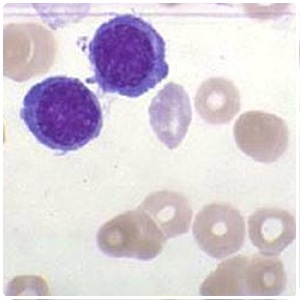
\includegraphics[scale=0.5]{erito.jpg}
      \caption{\tiny Eritroblastos, mobiliza parte de seu material genético para a sintese da hemoglobina, mas é incapaz de realizar outras funções metabolicas.}
    \end{figure} 
\end{frame}

\begin{frame}
  \frametitle{Controles e Fatores que Atuam na Diferenciação}
  \raggedright
    \begin{block}{Fatores que influenciam na Diferenciação:}
    \footnotesize 
	\begin{itemize}
	  \item Há fatores intracelulares, extracelulares e extrínsecos. Além, de fatores ambientais e agentes externos.
	\end{itemize}
    \end{block}
    \pause
    
    \begin{figure}
      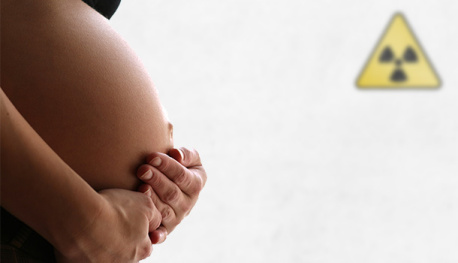
\includegraphics[scale=0.46]{gravidez_radiacao.jpg}
      \caption{\tiny A exposição da gestante a radiação provocada pelo Raio-X pode afetar no processo de diferenciação do feto.}
    \end{figure}    
\end{frame}

\begin{frame}
  \frametitle{Controles e Fatores que Atuam na Diferenciação}
  \raggedright
   \begin{block}{Irreversibilidade da Diferenciação:}
    \footnotesize 
	\begin{itemize}
	  \item Desprogramação celular: Regeneração
	\end{itemize}
    \end{block}

    \begin{figure}
      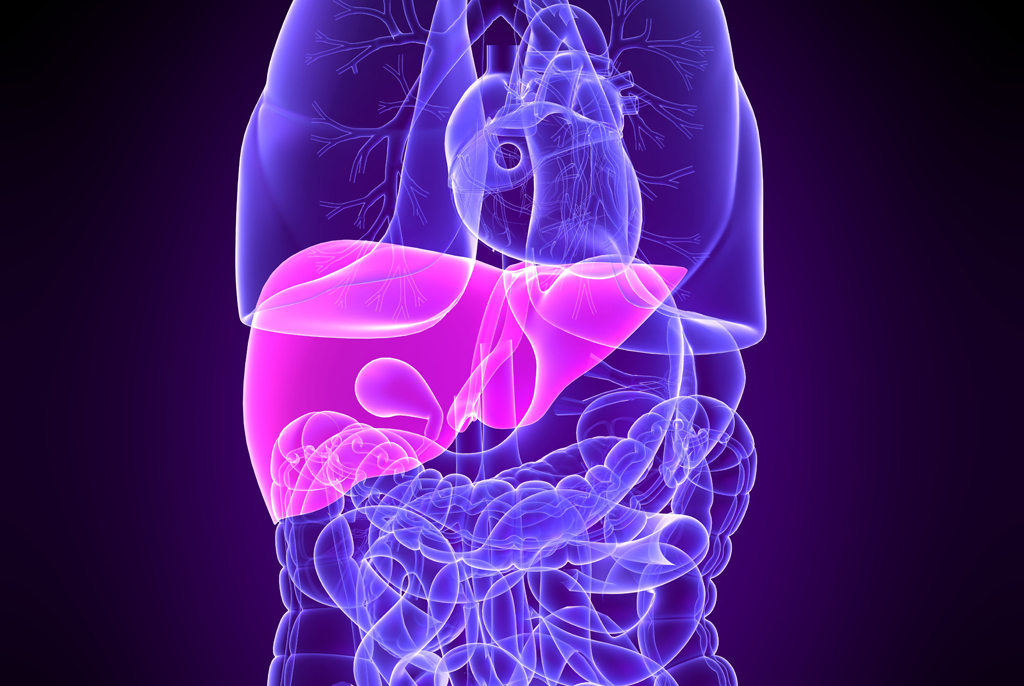
\includegraphics[scale=0.5]{regenera_figado.jpg}
      \caption{\tiny A regeneração do fígado é um Exemplo de Desprogramação Celular.}
    \end{figure}
\end{frame}

\begin{frame}
  \frametitle{Controles e Fatores que Atuam na Diferenciação}
  \raggedright
     \begin{block}{Diferenciação na fase }
    \footnotesize 
	\begin{itemize}
	    \item É comum acreditar que a diferenciação ocorre apenas na fase inicial do desenvolvimento.
	\end{itemize}
    \end{block}
    

    \pause
    \begin{figure}
        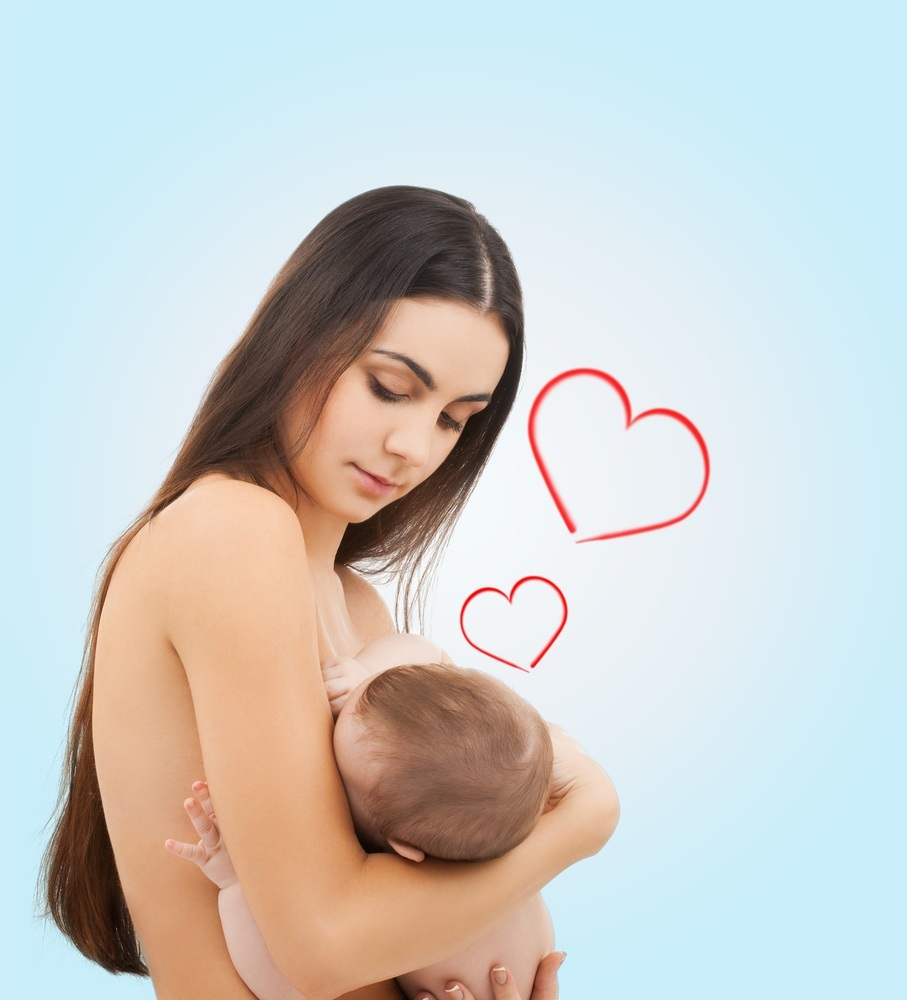
\includegraphics[scale=0.15]{amamentacao.jpg}
	\caption{\tiny A diferenciação das glândulas mamarias estaciona-se por um tempo e é retomada durante a gravidez.}
    \end{figure}
\end{frame}

%%%%%%%%%%%%%%%%%%%%%%%%%%%%%%%%%%%%%%%%%%%%%%%%%%%%%%%%%%%%%%%%%%%%%%%%%%%%%%%%%%%%%%%%%%%%%%%%%%%%%%%%%%%%%%%%%%%%%%%%%%%%%%%%%%%%%%%%%%%%%%%%%%%%%%%%%%%%%%%%%%%%%%%%%%%%%%%%
%%%%%%%%%%%%%%%%%%%%%%%%%%%%%%%%%%%%%%%%%%%%%%%%%%%%%%%%%%%%%%%%%%%%%%%%%%%%%%%%%%%%%%%%%%%%%%%%%%%%%%%%%%%%%%%%%%%%%%%%%%%%%%%%%%%%%%%%%%%%%%%%%%%%%%%%%%%%%%%%%%%%%%%%%%%%%%%%
\section{Clonagem}

\begin{frame}
\frametitle{Clonagens}

   \begin{block}{Desprogramação}
    \footnotesize 
	\begin{itemize}
	    \item A evolução das técnicas de desprogramação nuclear possibilitou a clonagem de mamíferos.
	\end{itemize}
   \end{block}
   \begin{figure}
      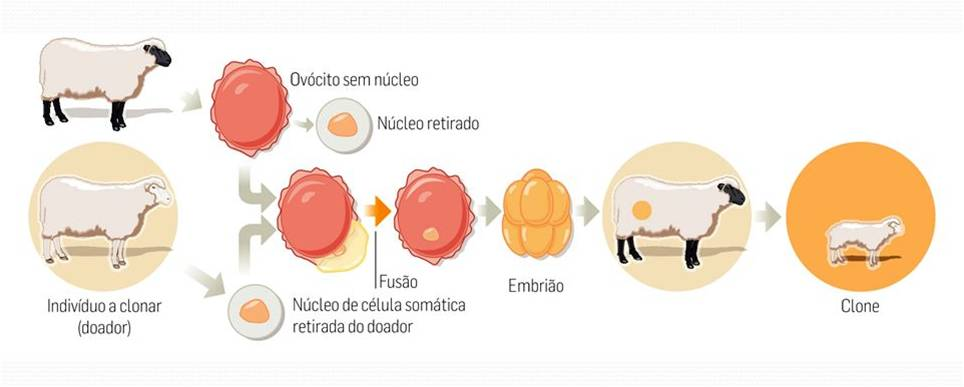
\includegraphics[scale=0.5]{clone.jpg}
      \caption{\tiny Clone Ovelha Dolly. Esse experimento demosntra que o núcleo transplantado continha todos os genes que estavam no zigotio.}
   \end{figure}
\end{frame}

%%%%%%%%%%%%%%%%%%%%%%%%%%%%%%%%%%%%%%%%%%%%%%%%%%%%%%%%%%%%%%%%%%%%%%%%%%%%%%%%%%%%%%%%%%%%%%%%%%%%%%%%%%%%%%%%%%%%%%%%%%%%%%%%%%%%%%%%%%%%%%%%%%%%%%%%%%%%%%%%%%%%%%%%%%%%%%%%
%%%%%%%%%%%%%%%%%%%%%%%%%%%%%%%%%%%%%%%%%%%%%%%%%%%%%%%%%%%%%%%%%%%%%%%%%%%%%%%%%%%%%%%%%%%%%%%%%%%%%%%%%%%%%%%%%%%%%%%%%%%%%%%%%%%%%%%%%%%%%%%%%%%%%%%%%%%%%%%%%%%%%%%%%%%%%%%%
\section{Perguntas}

\begin{frame}
  \frametitle{Perguntas}
  \begin{enumerate}
    \item Por quais motivos durante a gravidez deve ser evitado a exposição a radiações, como o Raio-X?
    \pause
    \begin{itemize}
     \item A exposição prolongada a radiações irá afetar o proceso de diferenciação do feto. 
    \end{itemize}

    \item O que faz uma mesma célula que tem capacidade multipotente se transformar em vários tipos de tecidos? 
    \pause 
    \begin{itemize}
     \item Devido a sua expreção génetica, o gêne que se expressa na multiplicação dessa célula vai variar e se expressar de forma diferente, formando tecidos diferentes. 
    \end{itemize}

    \end{enumerate}
  \begin{figure}
     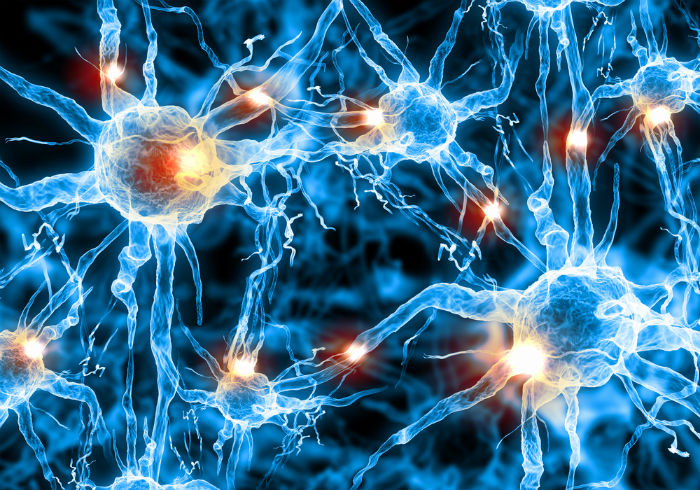
\includegraphics[scale=0.2]{perguntas.jpg}
  \end{figure}

\end{frame}

%%%%%%%%%%%%%%%%%%%%%%%%%%%%%%%%%%%%%%%%%%%%%%%%%%%%%%%%%%%%%%%%%%%%%%%%%%%%%%%%%%%%%%%%%%%%%%%%%%%%%%%%%%%%%%%%%%%%%%%%%%%%%%%%%%%%%%%%%%%%%%%%%%%%%%%%%%%%%%%%%%%%%%%%%%%%%%%%
%%%%%%%%%%%%%%%%%%%%%%%%%%%%%%%%%%%%%%%%%%%%%%%%%%%%%%%%%%%%%%%%%%%%%%%%%%%%%%%%%%%%%%%%%%%%%%%%%%%%%%%%%%%%%%%%%%%%%%%%%%%%%%%%%%%%%%%%%%%%%%%%%%%%%%%%%%%%%%%%%%%%%%%%%%%%%%%%
\section{Referências}
\begin{frame}
 \frametitle{Referências}
 \tiny
      \begin{enumerate}[1]
      \item Lodish, H. Biologia Celular e Molecular
      \item Junqueira, L, C. Biologia Celular e Molecular. 
      %% para verificar alteração no github
      \end{enumerate}
\end{frame}

\end{document}
